\documentclass{./../div_teaching_slides}

\begin{document}
\title{ECON 340 \\ Economic Research Methods}
\author{Div Bhagia}
\date{Lecture 16: Prediction vs. Causal Inference}

%%%%%%%%%%%% 
\begin{frame}[noframenumbering, plain]
\maketitle
\end{frame}

%%%%%%%%%%%%%%%%%%%%%%%%%% Review 

%%%%%%%%%%%% 
\begin{frame}{Ordinary Least Squares (OLS)}
What is the main goal of Ordinary Least Squares (OLS)? \\ \vspace{0.5em}
\begin{witemize}
  \item[(a)] Choose the line that passes through as many data points as possible
  \item[(b)] Choose the values for slope and intercept that minimize the sum of squared residuals
  \item[(c)] Choose the line that minimizes the absolute distance between the predicted values and data
  \end{witemize}
\end{frame}


%%%%%%%%%%%% 
\begin{frame}{Ordinary Least Squares (OLS)}
\begin{columns}[c]
\begin{column}{0.7\textwidth}
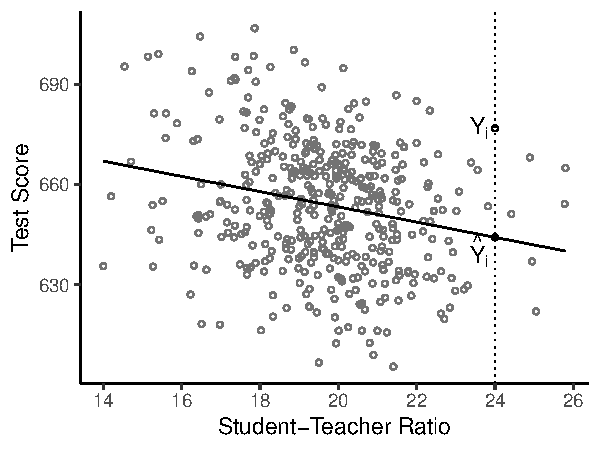
\includegraphics{./../../output/lrm_caschool_ols.pdf}
\end{column}
\begin{column}{0.35\textwidth}
Best fit line minimizes the sum of squared errors: $$\sum_{i=1}^n \hat{u}_i^2 =\sum_{i=1}^n(Y_i - \hat{Y}_i)^2$$
Fitted line:
$$ \hat{Y}_i = \hat{\beta}_0 + \hat{\beta}_1 X  $$
\vfill
\end{column}
\end{columns}
\end{frame}

%%%%%%%%%%%% 
\begin{frame}{Goodness of Fit: The $R^2$}
\begin{witemize}
\item[]   \textit{Total Sum of Squares:} $TSS = \sum_{i=1}^n (Y_i-\bar{Y})^2 $
\item[]  \textit{Explained Sum of Squares:} $  ESS = \sum_{i=1}^n (\hat{Y}_i-\bar{Y})^2 $
\item[]   \textit{Residual Sum of Squares:} $  RSS = \sum_{i=1}^n (Y_i-\hat{Y}_i)^2 =\sum_{i=1}^n \hat{u}_i^2$ \\~\\
\end{witemize}
$$ TSS = ESS + RSS $$ \\~\\
A measure of goodness of fit: 
$$ R^2 = \frac{ESS}{TSS} = 1-\frac{RSS}{TSS} $$
\end{frame}

%%%%%%%%%%%% 
\begin{frame}{Goodness of Fit: The $R^2$}
Are the following statements true or false? \\ \vspace{0.5em}
\begin{witemize}
  \item[(a)]  $R^2$ ranges from 0 to 1.
  \item[(b)] A higher $R^2$ indicates that the regression line is a better fit.
  \item[(c)] A higher $R^2$ indicates that $X$ explains a large percent of variation in $Y$.
  \item[(d)] If the slope $\hat{\beta_1}=0$, then $R^2=1$.
  \end{witemize}
\end{frame}

%%%%%%%%%%%% 
\begin{frame}{How to interpret the coefficients?}
Fitted line:
$$ \hat{testscr} = 698.93 -2.28 \cdot str $$
\pause 
\begin{witemize}
  \item Intercept: Predicted test score is 698.93 for a school with $str=0$. (Doesn't always make sense!)
  \item Slope: One more student per teacher lowers the predicted test score by 2.28. How? \\ \vspace{0.25em}
   \textit{Alternatively}: Schools in our sample that had one more student per teacher on average had an average test score that was 2.28 points lower.
\end{witemize}
\end{frame}

%%%%%%%%%%%%%%%%%%%%%%%%%% Review over

%%%%%%%%%%%% 
\begin{frame}{Two Different Questions}
\begin{witemize}
  \item I am trying to figure out what are the test scores for a particular school, but I can only observe it's class size. If my linear model captures the data well, I could use it to \textit{predict} the test score for this school.
  \item But now, what if the Department of Education wants to know whether reducing class size across schools will \textit{lead} to an improvement in test scores. Can my model answer this question?
\end{witemize}
\end{frame}

%%%%%%%%%%%% 
\begin{frame}{Two Different Questions}
\begin{witemize}
  \item First question concerns \textit{prediction}: using the observed value of some variable to predict the value of another variable
  \item The second concerns \textit{causal inference}: using data to estimate the \textit{effect} of changes in one variable on another variable
  \item To attach a causal interpretation to $\beta_1$, we need additional assumptions
\end{witemize}
\end{frame}

%%%%%%%%%%%% 
\begin{frame}{Simple Linear Regression Model}
\textit{Assumption 1 (Linearity):}
The relationship between $X$ and $Y$ is given by: 
$$ Y = \beta_0 + \beta_1 X + u $$
\vspace{1em}
Here, $u$ is the mean zero error term, $E(u)=0$. \\~\\
There is a linear (in parameters) relationship between $X$ and $Y$ with some error that is on average zero. \\~\\
Can think of $u$ as the impact of omitted factors on $Y$.
\end{frame}

%%%%%%%%%%%% 
\begin{frame}{Assumptions for Causal Inference}
\vspace{0.5cm}
\textit{Assumption 2 (Random Sample):} The observed data $(Y_i, X_i)$ for $i=1,2,...,n$ represent a random sample of size $n$ from the above population model. \\
\vspace{1.5cm}

\textit{Assumption 3 (No large outliers)}: Fourth moments (or Kurtosis) of $X$ and $Y$ are finite.
\end{frame}

%%%%%%%%%%%% 
\begin{frame}{Why we don't want outliers}
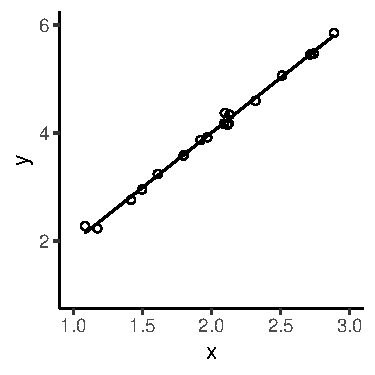
\includegraphics{./../../output/outliers_without.pdf}
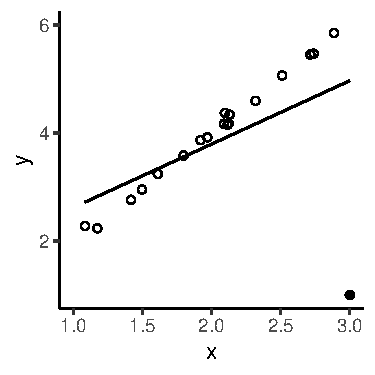
\includegraphics{./../../output/outliers_with.pdf}
\end{frame}


%%%%%%%%%%%% 
\begin{frame}{Assumptions for Causal Inference}
\vspace{0.5cm}
\textit{Assumption 4 (\textit{Mean Independence}/Exogeneity):} The expected value of the error term is the same conditional on any value of the explanatory variable.
$$ E(u|X)=E(u)=0 $$ \\~\\

This assumption is crucial for attaching a causal interpretation to our regression coefficients.
\end{frame}

%%%%%%%%%%%%% 
%\begin{frame}{Reminder: Conditional Expectation}
%Expectation: $$ E(Y) = \sum_y y \cdot f(y) $$
%Conditional probability: $$ f(y | x) = Pr(Y=y| X=x)$$
%Conditional expectation: $$ E(Y|X=x) = \sum_y y \cdot f(y|X=x) $$
%\end{frame}

%%%%%%%%%%%% 
\begin{frame}{\large Reminder: Independence and Uncorrelatedness}
\begin{witemize}
\item Two random variables are \textit{independent} if $ f(y|x) = f(y)$ for all $x$ and $y$ or equivalently $ E(Y|X) = E(Y)$. 
\item Two random variables are \textit{uncorrelated} if the correlation between them is 0. 
\item Independence $\rightarrow$ uncorrelatedness, if two variables are independent then they are uncorrelated as well
\end{witemize}
\end{frame}

%%%%%%%%%%%%
\begin{frame}{The Exogeneity Assumption}
$$ Y = \beta_0 + \beta_1 X + u \quad \quad Exogeneity: E(u|X) = E(u) = 0$$ 
\begin{witemize}
  \item Omitted factors do not dependent on values of $X$
  \item In other words, the error term is uncorrelated with the independent variable $X$ 
  \item Why do we need this assumption to attach a causal interpretation to $\beta_1$?
\end{witemize}
\end{frame}

%%%%%%%%%%%% 
\begin{frame}{When the exogeneity assumption fails}
$$ Y = \beta_0 + \beta_1 X + u $$ \\ \vspace{0.5em}
\begin{witemize}
\item $Y$: test scores, $X$: class-size, $u:$ teacher quality
 \item If schools with higher student-teacher ratios have worse teachers ($ \uparrow X, \downarrow u$)
 \item Then, if we see test scores decline with class size ($ \uparrow X, \downarrow Y$), hard to say if it's due to teacher quality or class size.
\end{witemize}
\end{frame}

%%%%%%%%%%%% 
\begin{frame}{The Exogeneity Assumption}
\vspace{-1em}
$$ Y = \beta_0 + \beta_1 X + u $$ \\ \vspace{0.5em}
Let's take the expectation of $Y$ conditional on $X$: 
$$ E(Y | X) = \beta_0 + \beta_1 X + E(u|X) $$ \\ \vspace{0.5em}
If the exogeneity assumption holds, $E(u|X)=0$, then
$$ E(Y | X) = \beta_0 + \beta_1 X  $$ \\ \vspace{0.5em}
So change in $Y$ in response to one unit change in $X$, $$  E(Y | X=x+1)  -  E(Y | X=x) =  \beta_1 $$
\end{frame}



%%%%%%%%%%%% 
\begin{frame}{When the exogeneity assumption fails}
\vspace{-1.5em}
\begin{align}
	 & E(Y|X=x) = \beta_0 + \beta_1 x + E(u|X=x) \\ 
	 & E(Y|X=x+1) = \beta_0 + \beta_1 (x+1) + E(u|X=x+1) 
\end{align} \\~\\
Subtracting equation (1) from (2):
$$ E(Y|X=x+1)-E(Y|X=x) = \beta_1 + \underbrace{[E(u|X=x+1)-E(u|X=x)]}_{\text{Confounding effect of $u$}} $$ \\~\\
\end{frame}

%%%%%%%%%%%% 
\begin{frame}{Linear Regression Model}
Assumptions 1-4 imply that: \\~\\
\begin{enumerate}
  \item OLS estimators are unbiased, that is
$$ E(\hat{\beta_0}) = \beta_0, \quad  E(\hat{\beta_1}) = \beta_1 $$ 
\item In large samples, OLS estimators are normally distributed due to the Central Limit Theorem (CLT)
\end{enumerate}
\end{frame}
  
%%%%%%%%%%%% 
\begin{frame}{Sampling Distribution for OLS Estimators}
Under Assumptions 1-4, in large samples ($n>100$), 
 $$ \hat{\beta_0} \sim N(\beta_0, \sigma^2_{\hat{\beta_0}}), \quad \quad  \hat{\beta_1} \sim N(\beta_1, \sigma^2_{\hat{\beta_1}}) $$
 
 where $$ \sigma^2_{\hat{\beta}_1} = \frac{1}{n} \frac{Var[(X_i-\mu_X)u_i]}{Var(X_i)} $$	\pause \\~\\

 Can you think why the variance of $\hat{\beta}_1$ decreases as the variance of $X$ increases?
\end{frame}

%%%%%%%%%%%% 
\begin{frame}{Variance of $\hat{\beta}_1$ and $X$}
\centering
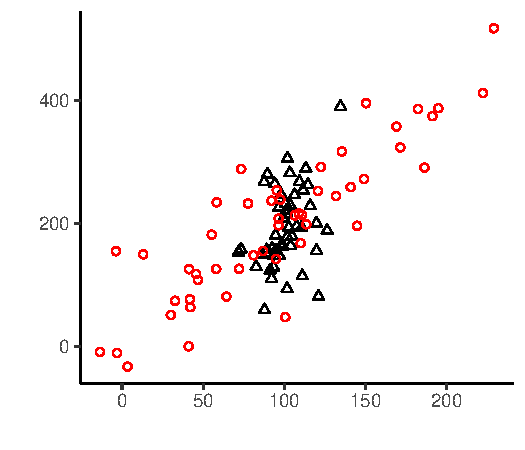
\includegraphics{./../../output/lrm_variance.pdf}
\end{frame}


%%%%%%%%%%%%% 
%\begin{frame}{Taking Stock}
%\begin{witemize}
%  \item Continue with regression analysis for the rest of the semester
%  \item Research Paper Submission 2 due on 10/31. Look at the instructions and start working on it if you haven't already.
%  \item Changed order of topics for the upcoming weeks on the syllabus (might need readjusting)
%\end{witemize}
%\end{frame}


\end{document}